\documentclass{beamer}

\usefonttheme{professionalfonts} % using non standard fonts for beamer
\usefonttheme{serif} % default family is serif

\usepackage{hyperref}
%\usepackage{minted}
\usepackage{animate}
\usepackage{graphicx}
\def\Put(#1,#2)#3{\leavevmode\makebox(0,0){\put(#1,#2){#3}}}
\usepackage{color}
\usepackage{tikz}
\usepackage{amssymb}
\usepackage{enumerate}


\newcommand\blfootnote[1]{%

  \begingroup

  \renewcommand\thefootnote{}\footnote{#1}%

  \addtocounter{footnote}{-1}%

  \endgroup

}

\makeatletter

%%%%%%%%%%%%%%%%%%%%%%%%%%%%%% Textclass specific LaTeX commands.

 % this default might be overridden by plain title style

 \newcommand\makebeamertitle{\frame{\maketitle}}%

 % (ERT) argument for the TOC

 \AtBeginDocument{%

   \let\origtableofcontents=\tableofcontents

   \def\tableofcontents{\@ifnextchar[{\origtableofcontents}{\gobbletableofcontents}}

   \def\gobbletableofcontents#1{\origtableofcontents}

 }

%%%%%%%%%%%%%%%%%%%%%%%%%%%%%% User specified LaTeX commands.

\usetheme{Malmoe}

% or ...

\useoutertheme{infolines}

\addtobeamertemplate{headline}{}{\vskip2pt}

\setbeamercovered{transparent}

% or whatever (possibly just delete it)

\makeatother

\begin{document}
\title[PFLOCK report]{PFLOCK Report}
\author[AC]{Andres Calderon}
\institute[Summer'19]{University of California, Riverside}
\makebeamertitle
\newif\iflattersubsect

\AtBeginSection[] {
    \begin{frame}<beamer>
    \frametitle{Outline} 
    \tableofcontents[currentsection]  
    \end{frame}
    \lattersubsectfalse
}

\AtBeginSubsection[] {
    \begin{frame}<beamer>
    \frametitle{Outline} 
    \tableofcontents[currentsubsection]  
    \end{frame}
}

\begin{frame}{Remarks of Chen et al. (2019)}
Real-time Distributed Co-Movement Pattern Detection on Streaming Trajectories (Chen et al., 2019)
    \begin{itemize}
        \item Explore a general co-movement pattern definition (following Fan et al, 2016) based on 5 constrains:
        \begin{enumerate}
            \item Closeness: control spatial proximity.
            \item Significance (M): control minimum number of objects.
            \item Duration (K): control how long objects move together.
            \item Consecutiveness (L): Minimum length of consecutive \textit{segments}.
            \item Connection (G): Maximum length of gaps between \textit{segments}.
        \end{enumerate}
    \end{itemize}
\end{frame}

\begin{frame}{Processing flow}
    \begin{enumerate}
        \item First, It focus on transforming the input on discretized snapshots (time instants).
        \begin{itemize}
            \item It uses window operations and time synchronization to organize locations happening at the same time.
        \end{itemize}
        \item Then, It focus on finding spatial cluster: 
        \begin{itemize}
            \item It uses closeness ($\varepsilon$) and significance (M) to run DBSCAN and find cluster at each snapshot.
        \end{itemize}
        \item Finally, It focus on enumerating patterns in the temporal domain:
        \begin{itemize}
            \item It uses duration(K), consecutiveness (L) and connection (G) to mine set of clusters that fill those constrains. 
        \end{itemize}
    \end{enumerate}
\end{frame}

\begin{frame}{\underline{I}ndexed \underline{C}lustering and \underline{P}attern \underline{E}numeration}
    \centering 
    \begin{figure}
        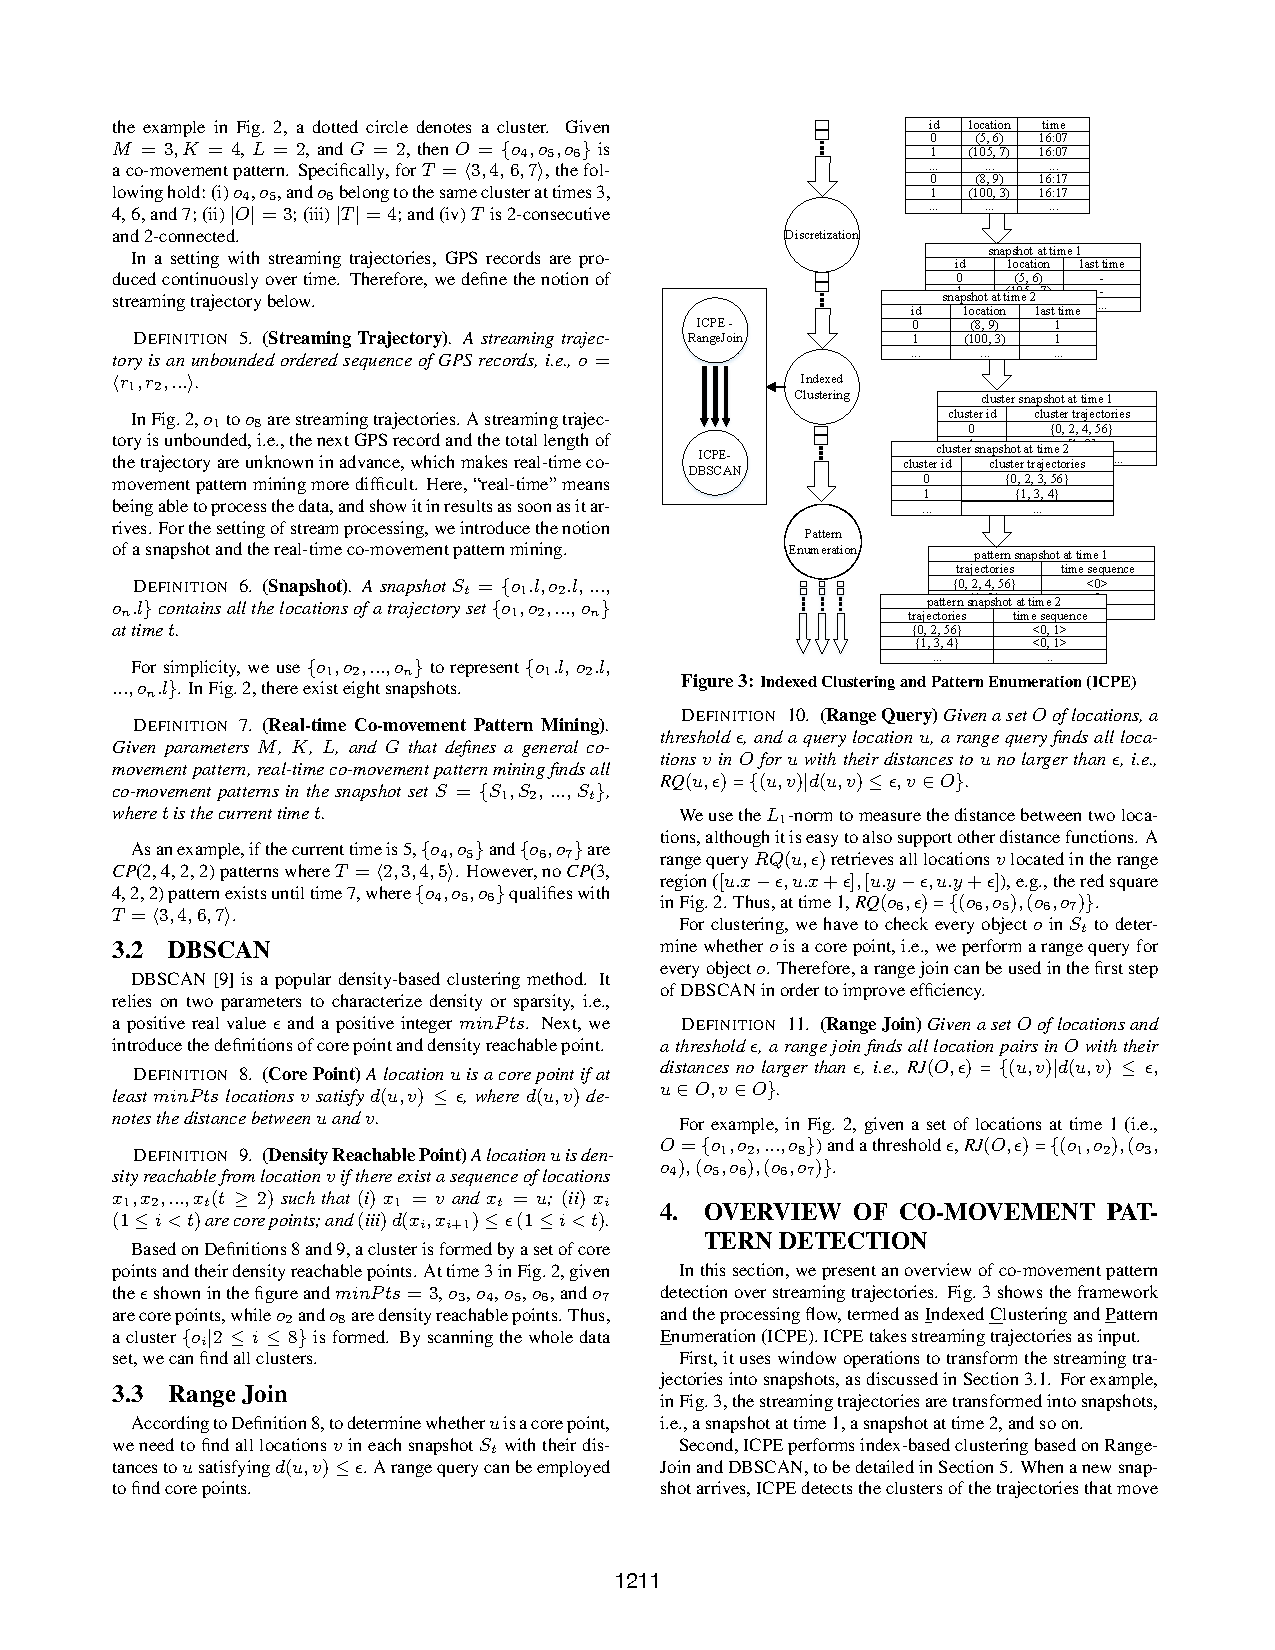
\includegraphics[trim=11cm 16.7cm 1.5cm 2cm, clip, width=0.6\textwidth]{figures/Chen_p1211}
    \end{figure}
\end{frame}

\begin{frame}{Indexed Clustering}
    \centering 
    \begin{figure}
        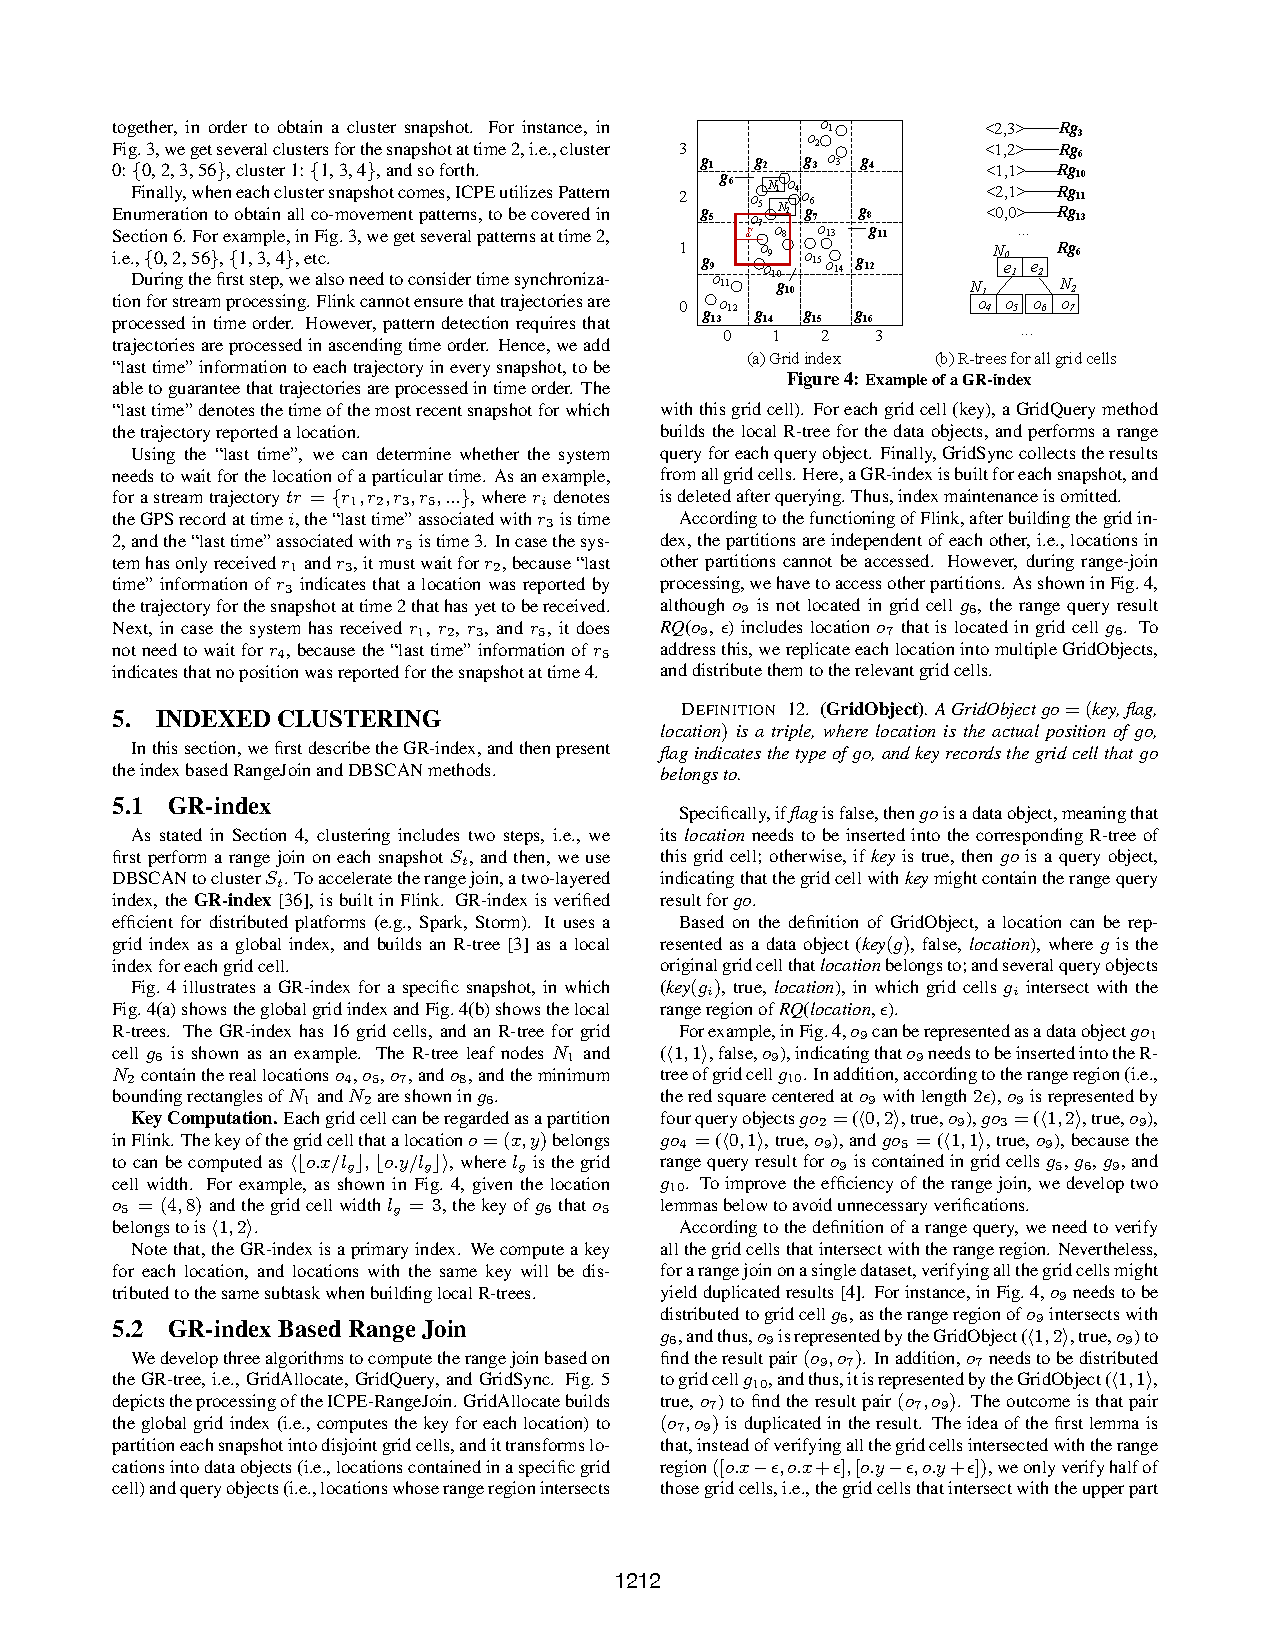
\includegraphics[trim=11cm 21.25cm 1.5cm 2cm, clip, width=.85\textwidth]{figures/Chen_p1212}
        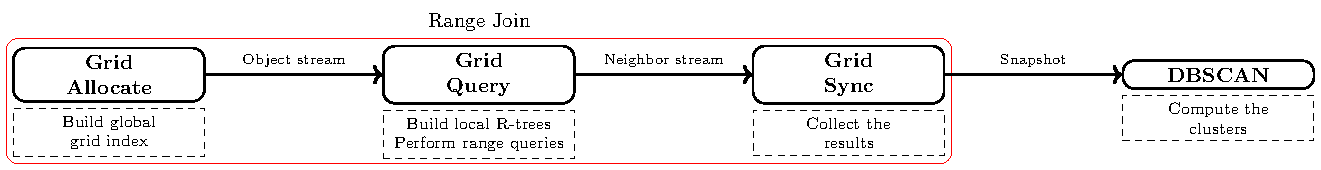
\includegraphics[width=1\textwidth]{figures/RangeJoin}
    \end{figure}
\end{frame}

\begin{frame}{Main diferences with our approach}
    \begin{itemize}
        \item DBSCAN finds variable shape clusters. Flocks demands disks with fixed diameter which introduce a large number of redundant/duplicate candidates.
        \item DBSCAN queries only input locations to find core and distance-reachable points.  Finding disk locations for flocks is more complex (twice the number of pairs).
        \item DBSCAN is run at Snapshot level, they claim Range Join prune enough points and partitions are no needed. ``In ICPE framework, we achieve the parallelism by clustering snapshots separately.'' It depends in dataset size and parameters.
    \end{itemize}
\end{frame}

\begin{frame}{Pattern Enumeration}
    \centering 
    \begin{figure}
        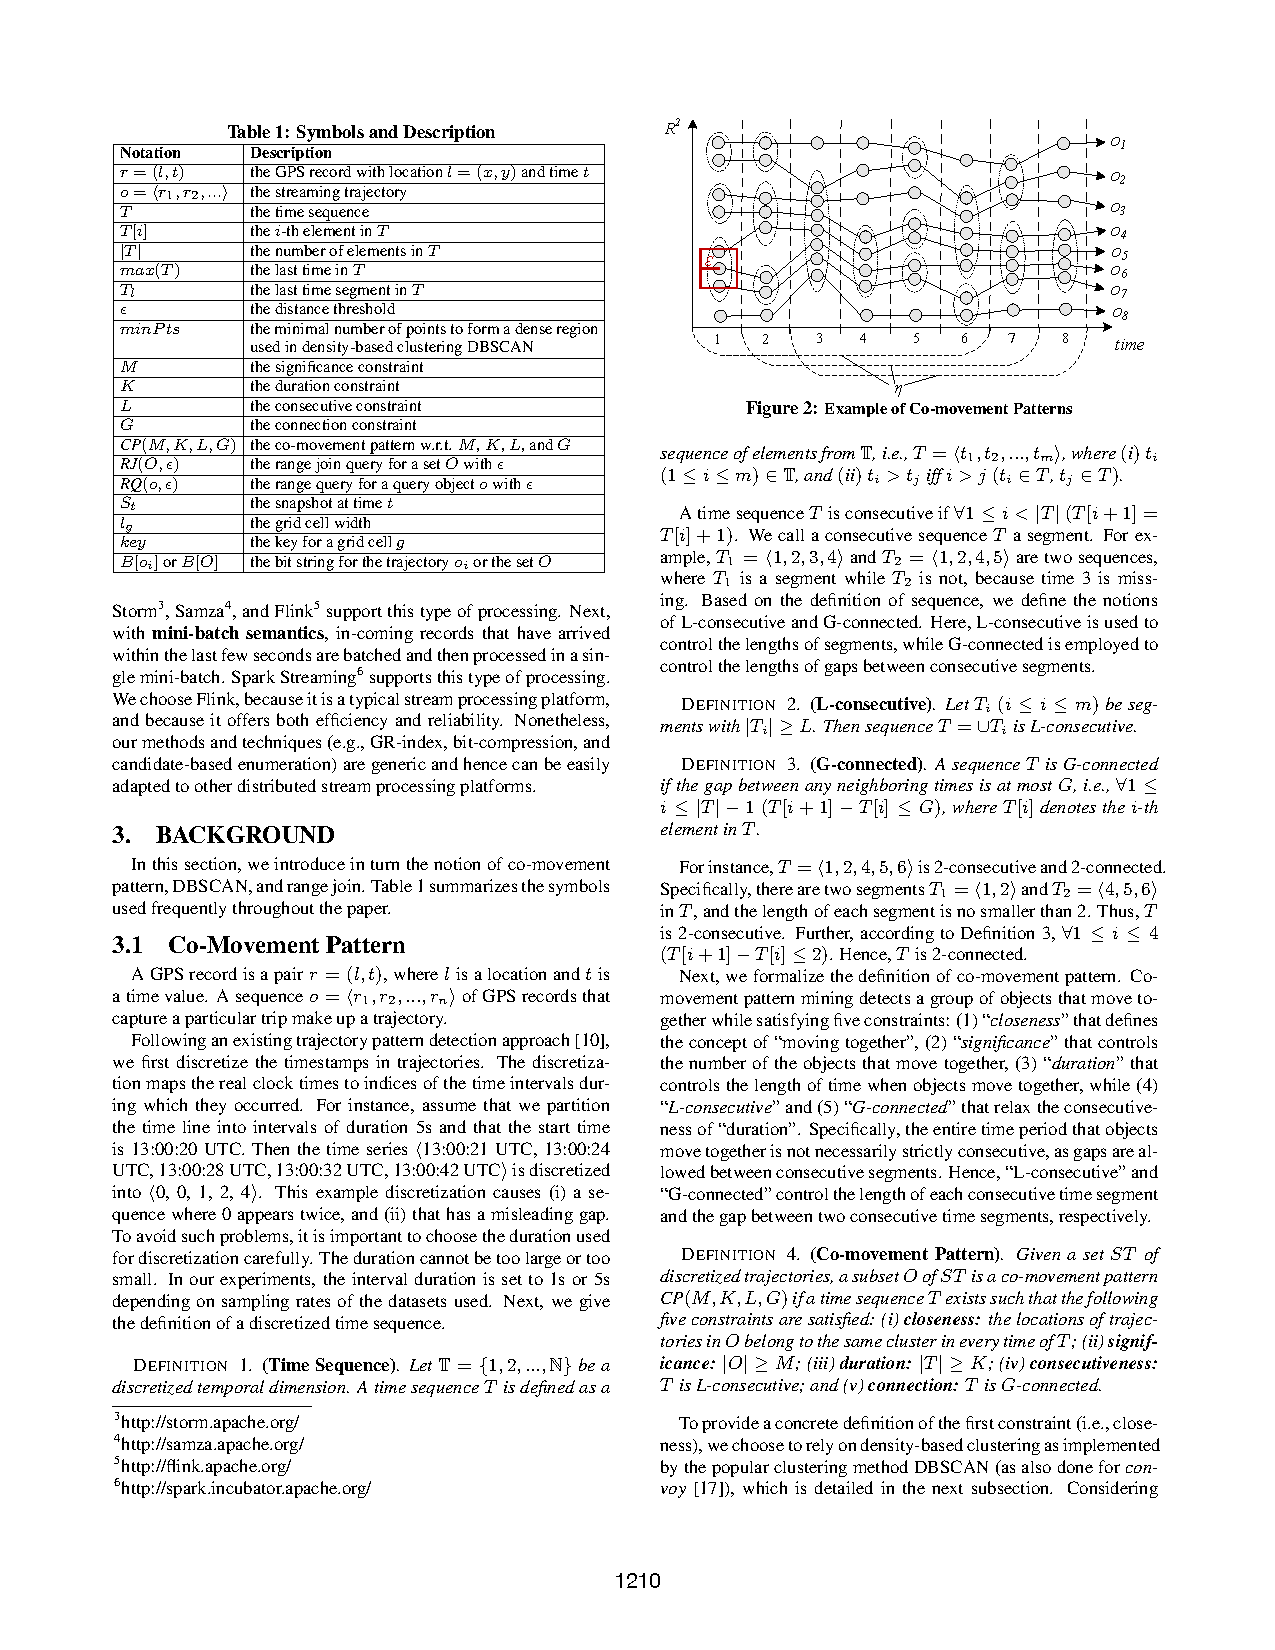
\includegraphics[trim=11cm 21.25cm 2cm 2cm, clip, width=\textwidth]{figures/Chen_p1210}
    \end{figure}
\end{frame}

\begin{frame}{Partitions on temporal domain}
    \centering 
    \begin{figure}
        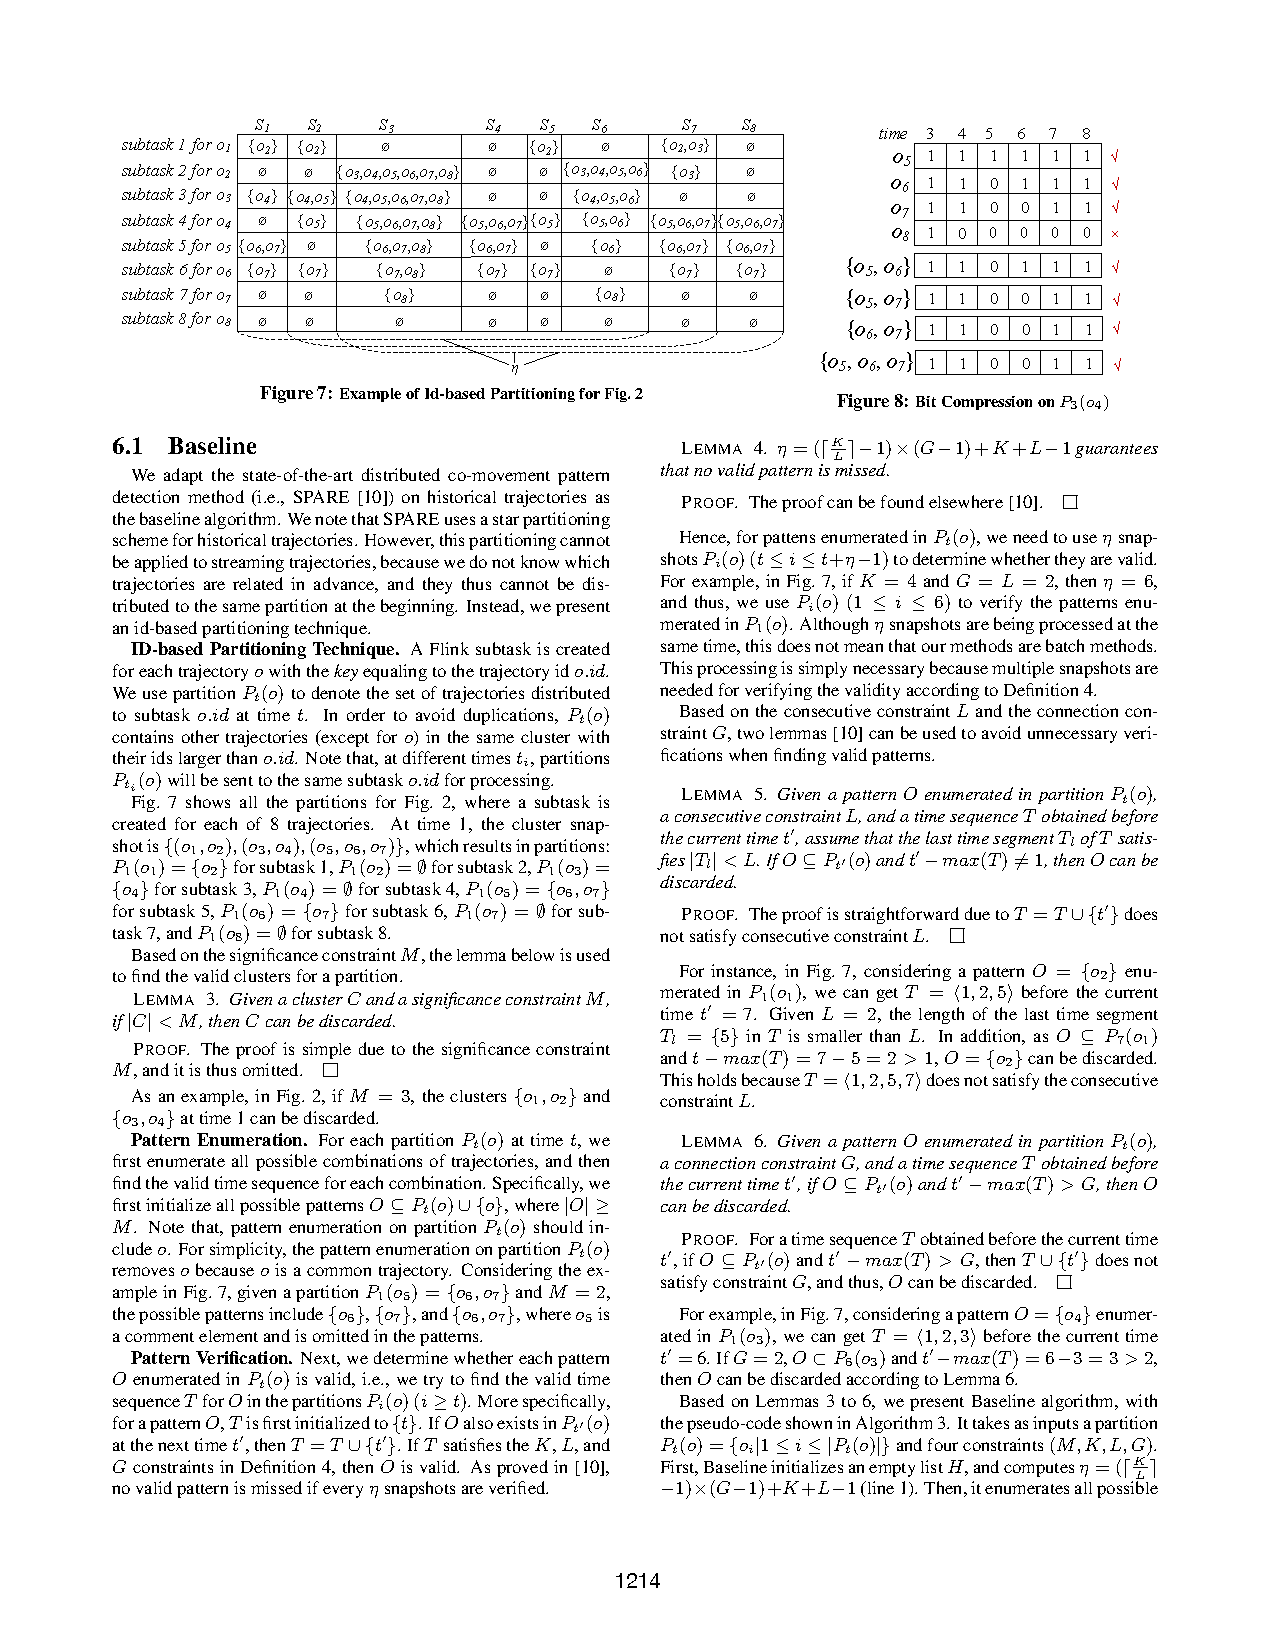
\includegraphics[trim=2cm 21cm 8cm 2cm, clip, width=1\textwidth]{figures/Chen_p1214}
    \end{figure}
    Fan et al. states and proves $\eta = (\lceil \frac{K}{L} - 1 \rceil) \times (G - 1) + K + L - 1$
\end{frame}

\begin{frame}{Pattern verification}
    \begin{enumerate}
        \item Baseline:
        \begin{itemize}
            \item For each $P_t(o)$ at time $t$, it enumerate all possible combinations ${o} \cup P_t(o)$.
            \item Then, it find the valid time sequence for each combination in the subsequent $\eta$ snapshots.
            \item i.e. for $P_2(o_3)= \{o_4,o_5\}$, it looks if $\{o_3,o_4\},\{o_3,o_5\},\{o_3,o_4,o_5\}$ appear in the following snapshots.
        \end{itemize}
    \end{enumerate}
\end{frame}

\begin{frame}{Bit compression improvements}
    \begin{enumerate}[2]
        \item Fixed Length Bit Compression Method:
    \end{enumerate}
    \centering 
    \begin{figure}
        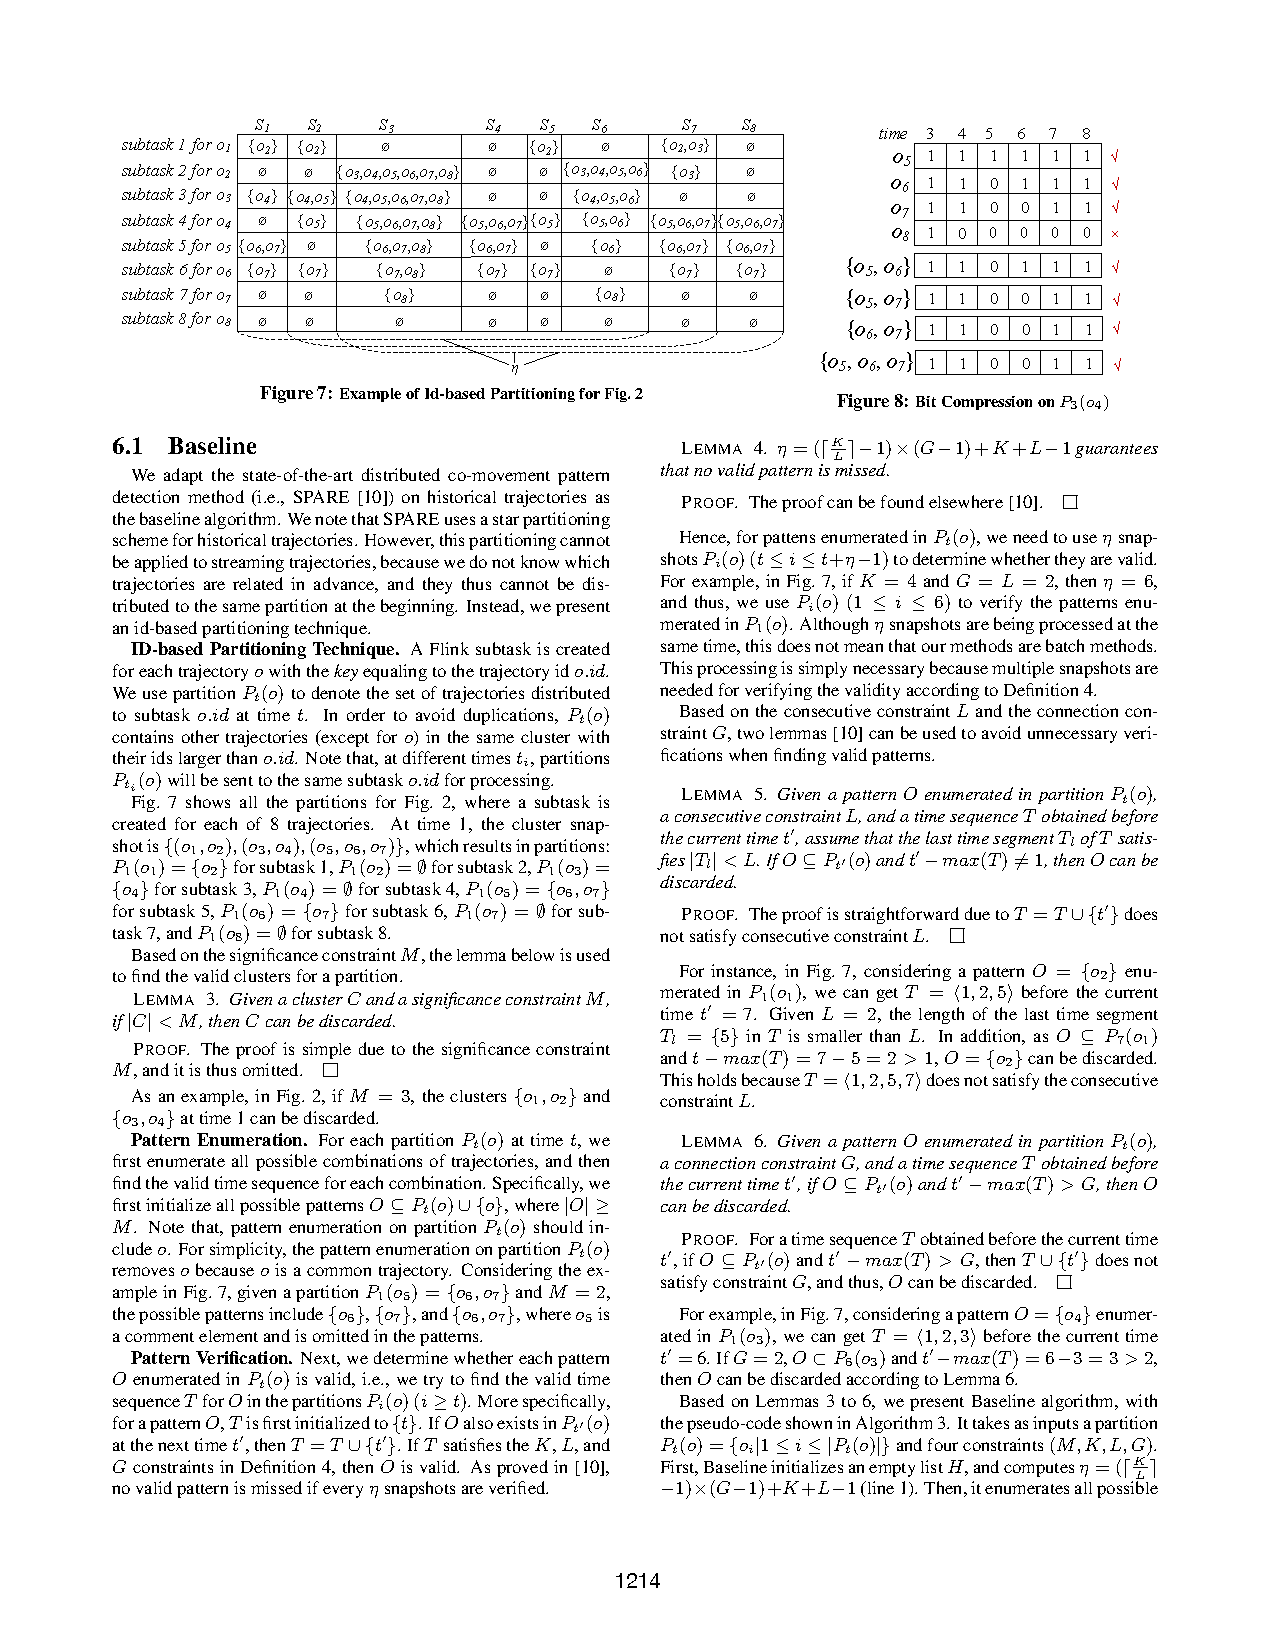
\includegraphics[trim=13.5cm 21cm 2cm 2cm, clip, width=0.6\textwidth]{figures/Chen_p1214}
    \end{figure}
\end{frame}

\begin{frame}{Bit compression improvements}
    \begin{enumerate}[3]
        \item Variable Length Bit Compression Method:
    \end{enumerate}
    \centering 
    \begin{figure}
        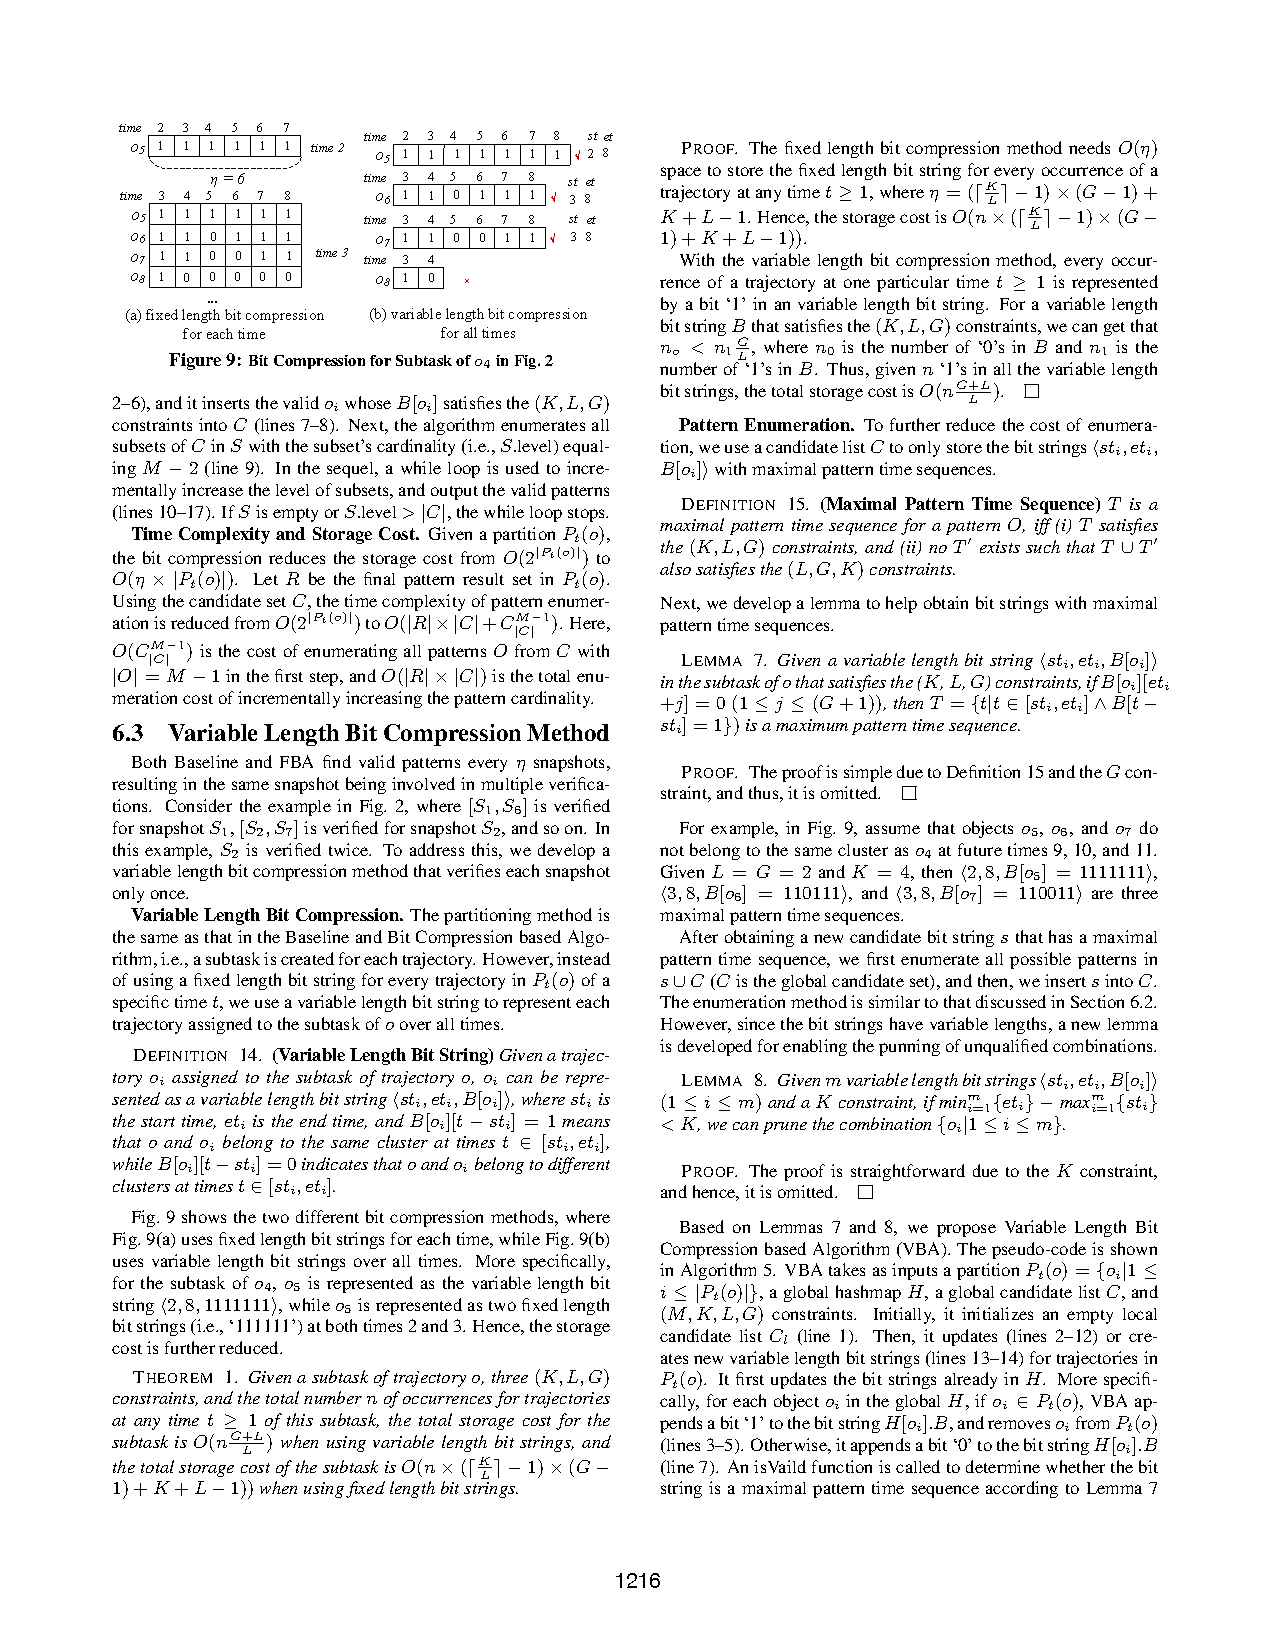
\includegraphics[trim=2cm 21.5cm 11.2cm 2cm, clip, width=0.9\textwidth]{figures/Chen_p1216}
    \end{figure}
\end{frame}

\begin{frame}{Experimental Evaluation}
    \centering
    \begin{figure}
        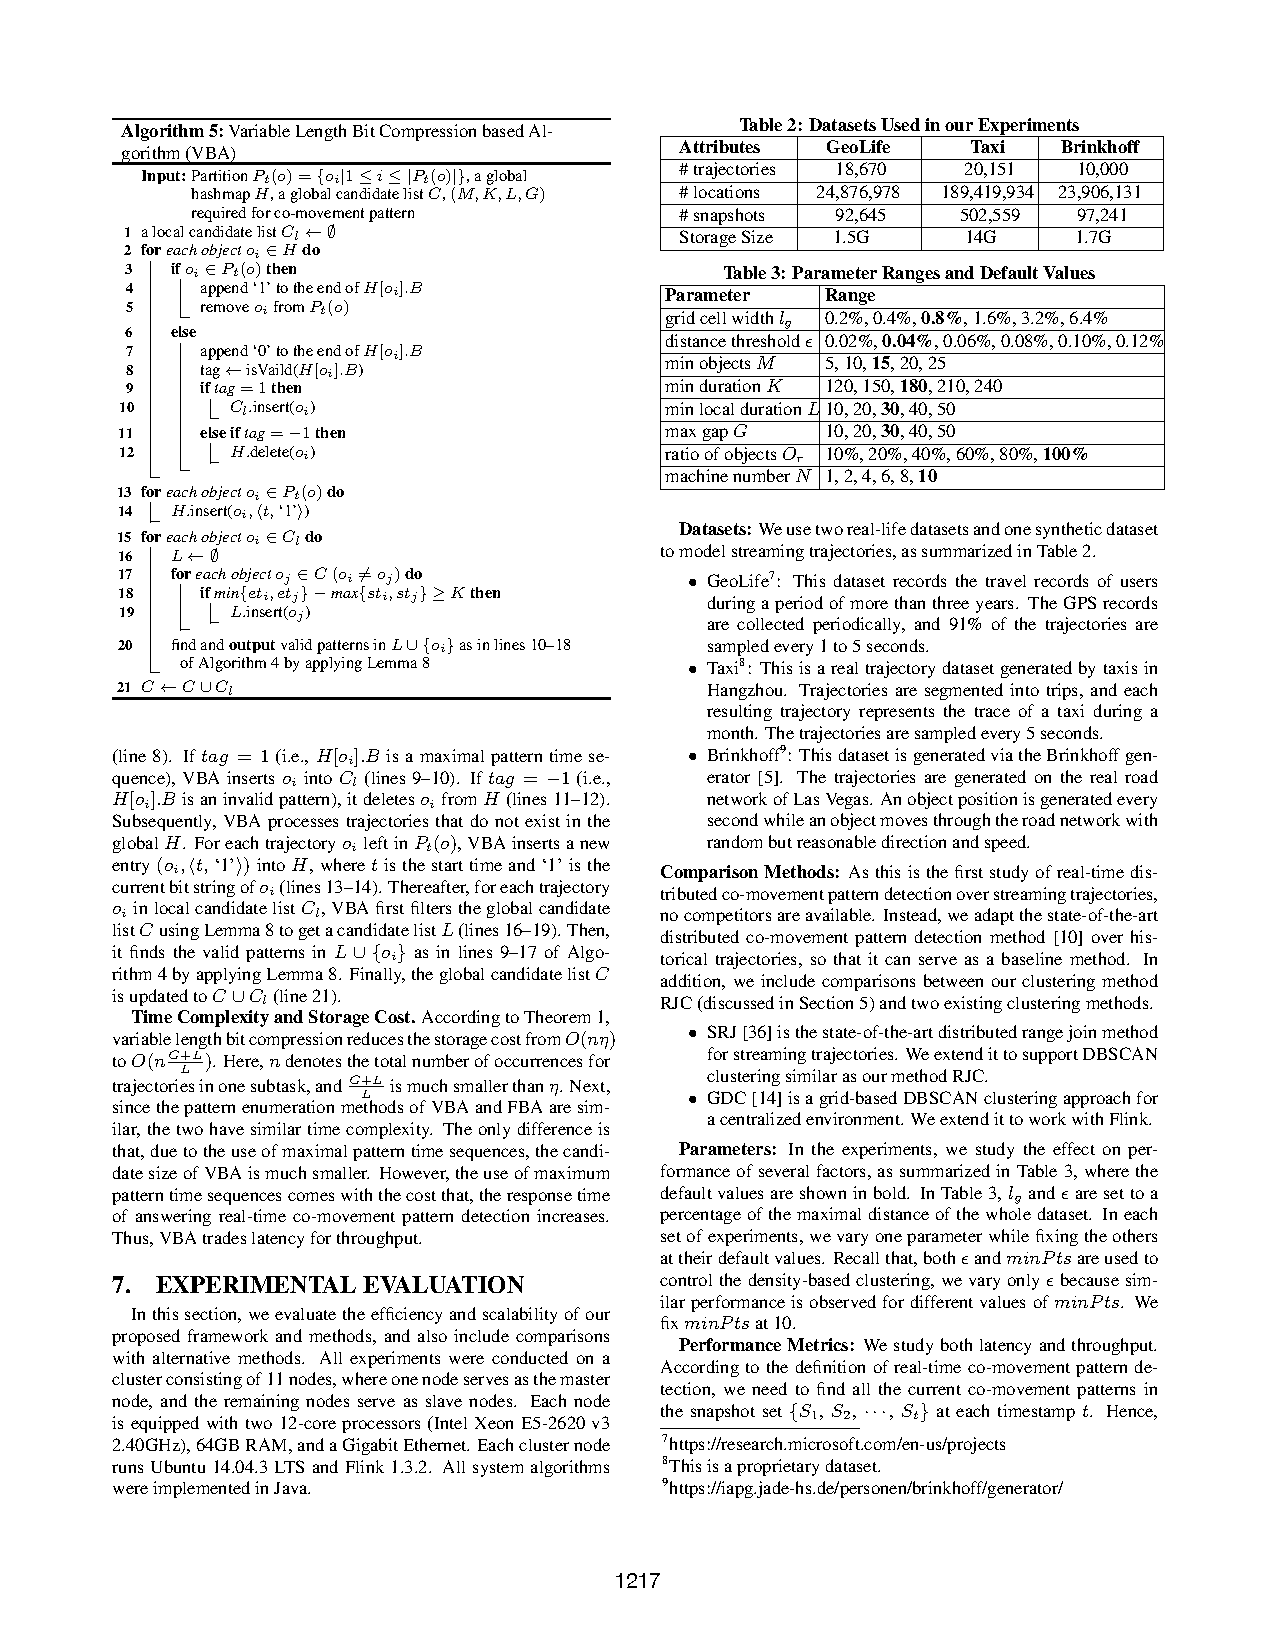
\includegraphics[trim=11cm 23.5cm 1.5cm 2cm, clip, width=1\textwidth]{figures/Chen_p1217}
    \end{figure}
    \blfootnote{\tiny{Locations per snapshot: GeoLife =  269, Taxi = 377, Brinkhoff = 246}}
\end{frame}

\begin{frame}{Experimental Evaluation}
    \centering
    \begin{figure}
        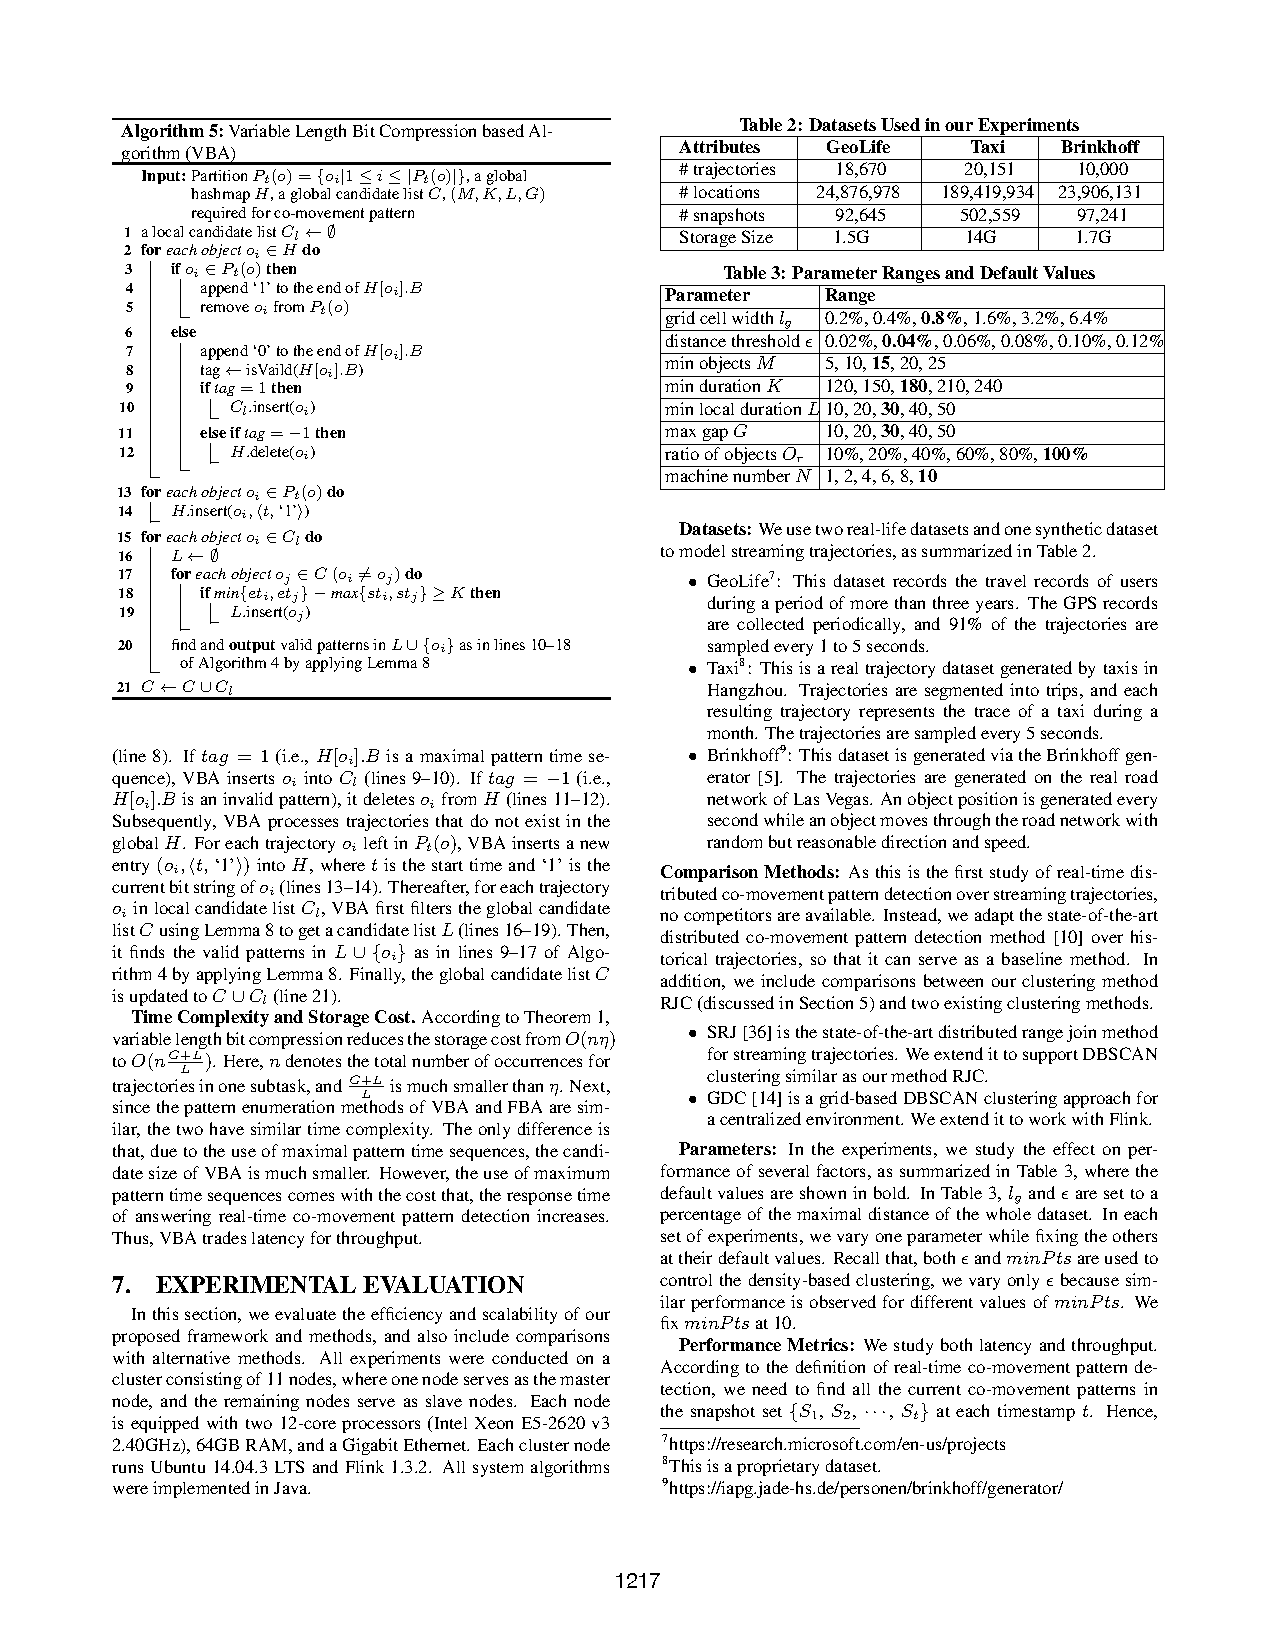
\includegraphics[trim=11cm 19.5cm 1.5cm 4.3cm, clip, width=1\textwidth]{figures/Chen_p1217}
    \end{figure}
    \blfootnote{\tiny{$l_g$ and $\epsilon$ are based on ``the maximal distance of the whole dataset'' (?)}}
\end{frame}

\begin{frame}{Experimental Evaluation}
    \centering
    \begin{figure}
        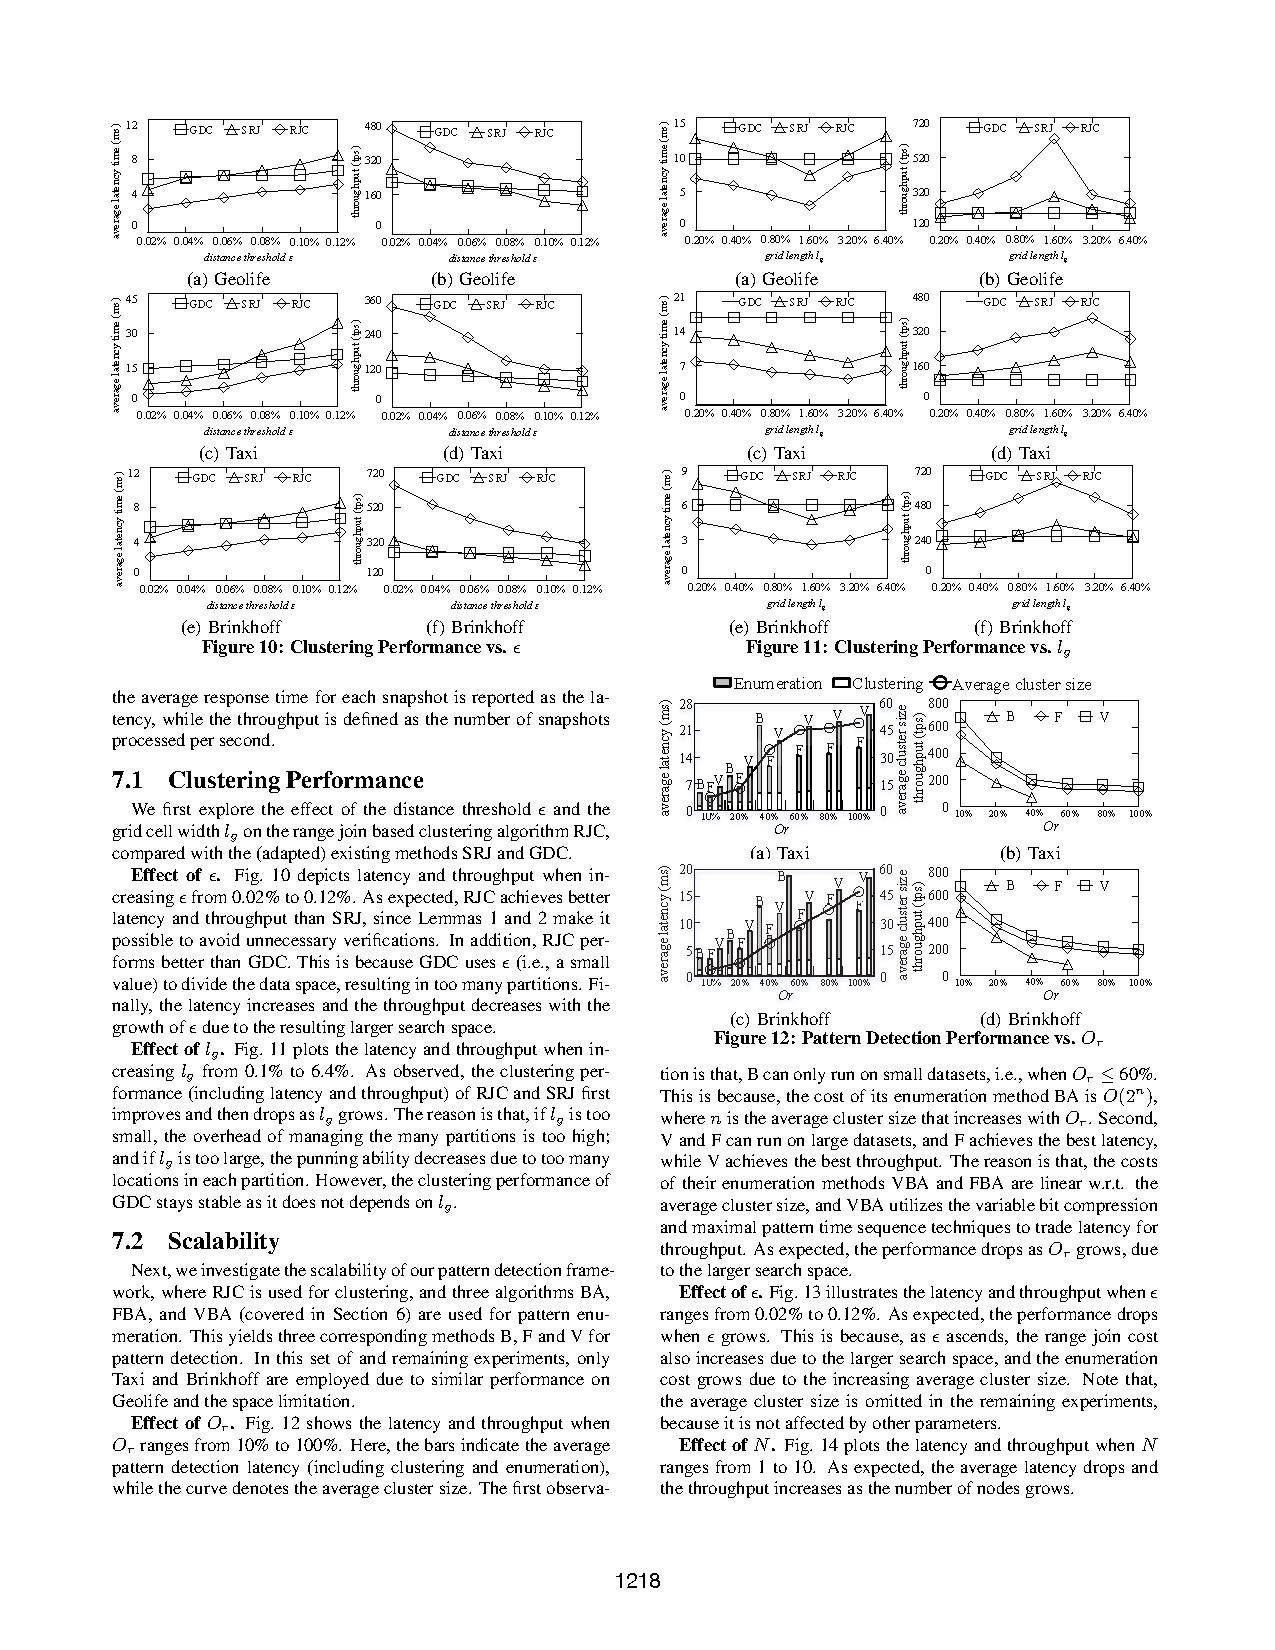
\includegraphics[trim=1.8cm 17.15cm 11.5cm 2cm, clip, width=0.525\textwidth]{figures/Chen_p1218}
    \end{figure}
    \blfootnote{\tiny{GDC: Grid-based DBSCAN Clustering, SRJ: state-of-the-art distributed range join.}}
\end{frame}

\begin{frame}{Experimental Evaluation}
    \centering
    \begin{figure}
        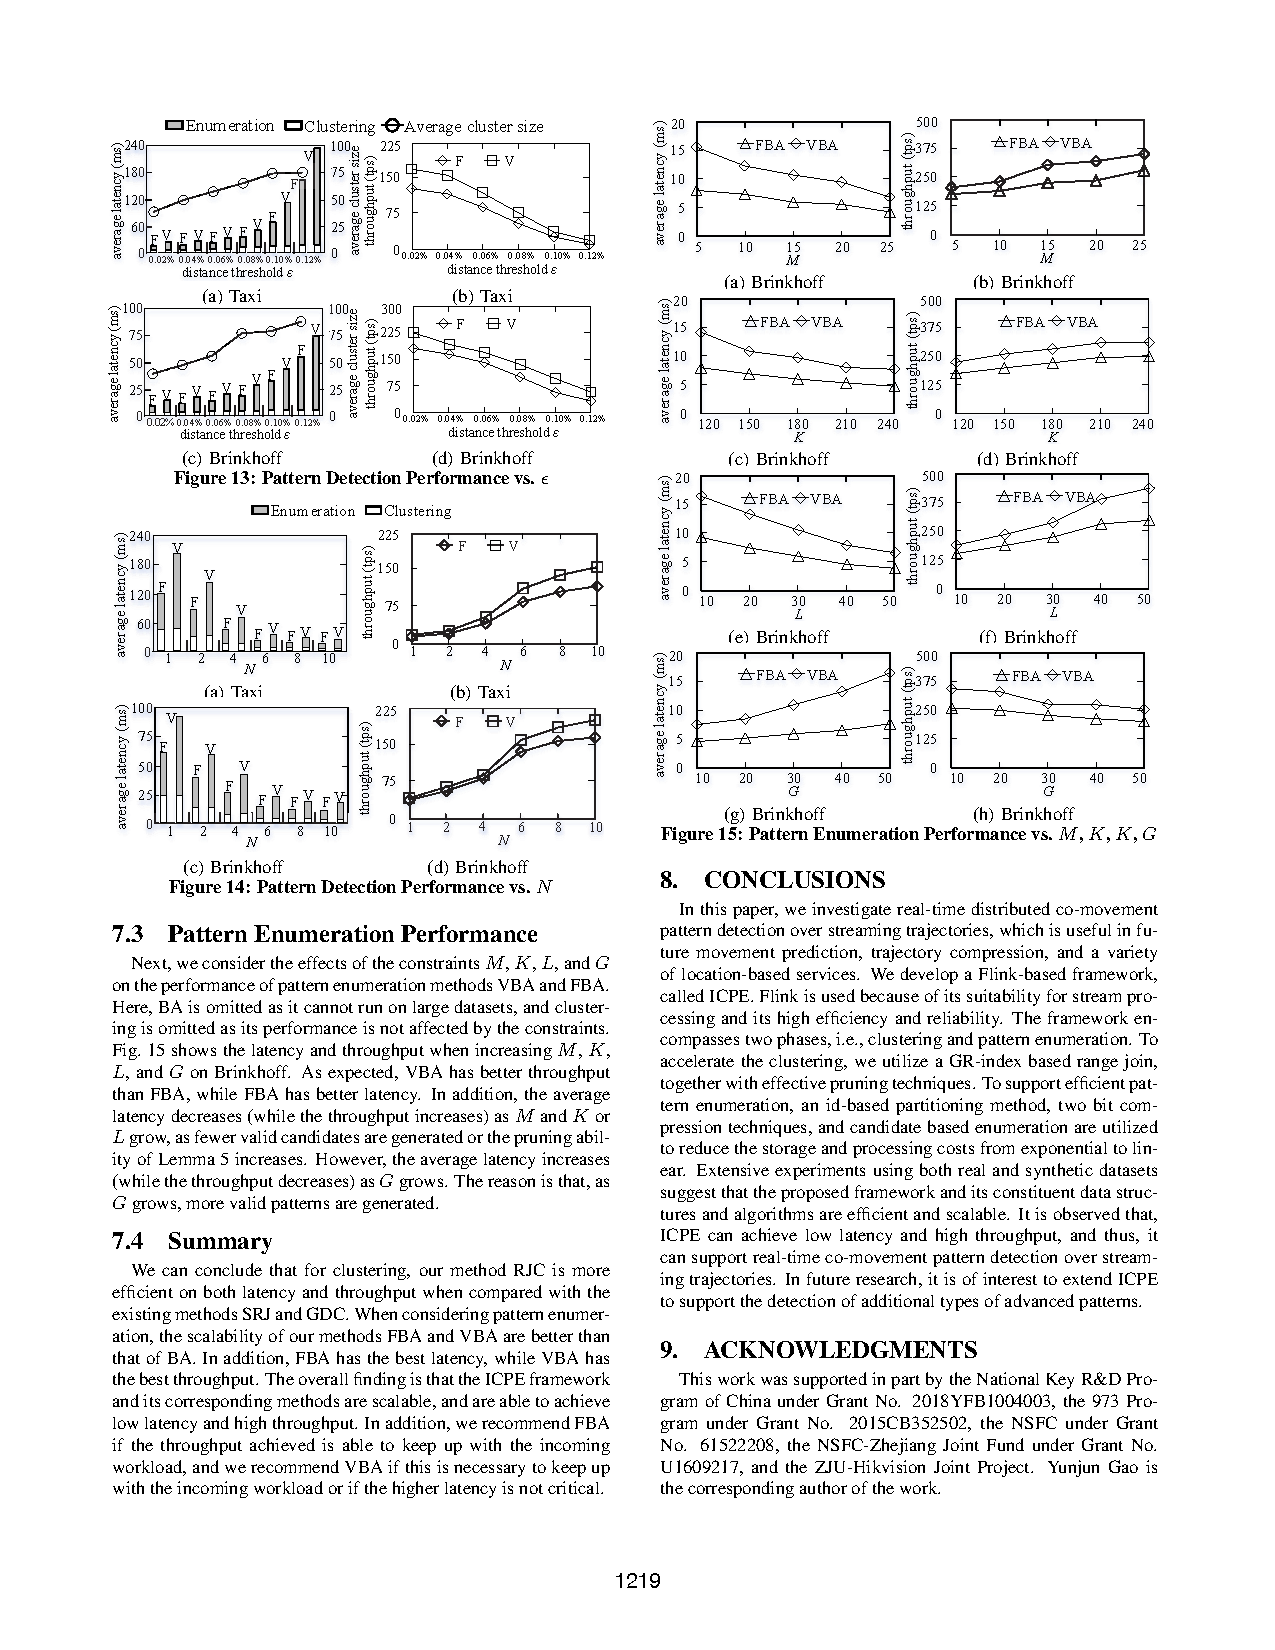
\includegraphics[trim=1.8cm 12.5cm 11cm 8.5cm, clip, width=0.65\textwidth]{figures/Chen_p1219}
    \end{figure}
    \blfootnote{\tiny{24 cores and 64Gb RAM per node}}
\end{frame}

\end{document}
